\documentclass[11pt]{article}

% ------------------------------------------------------------------
% Packages
% ------------------------------------------------------------------
\usepackage[letterpaper,margin=1in]{geometry}
\usepackage[T1]{fontenc}
\usepackage[scaled=0.95]{helvet}
\renewcommand{\familydefault}{\sfdefault}
\usepackage{amssymb}
\usepackage{xcolor}
\usepackage{tikz}
\usetikzlibrary{positioning,arrows.meta,shapes.geometric,fit,backgrounds,calc}
\usepackage{booktabs}
\usepackage{tabularx}
\usepackage{array}
\usepackage{enumitem}
\usepackage{listings}
\usepackage{fancyhdr}
\usepackage{titlesec}
\usepackage[most]{tcolorbox}
\usepackage[hidelinks]{hyperref}
\usepackage{graphicx}

% ------------------------------------------------------------------
% Colors & styles
% ------------------------------------------------------------------
\definecolor{patient}{HTML}{2E7D6B}
\definecolor{patientbg}{HTML}{E3F2EE}
\definecolor{clinic}{HTML}{2F4F8F}
\definecolor{clinicbg}{HTML}{E4EAF6}
\definecolor{backend}{HTML}{5A5A5A}
\definecolor{backendbg}{HTML}{F2F2F2}
\definecolor{model}{HTML}{8A4FA3}
\definecolor{modelbg}{HTML}{F1E7F6}
\definecolor{danger}{HTML}{B3261E}
\definecolor{dangerbg}{HTML}{FBE6E4}
\definecolor{store}{HTML}{9A6B12}
\definecolor{storebg}{HTML}{FBF1DC}
\definecolor{ink}{HTML}{222222}

\color{ink}
\setlist{itemsep=2pt,topsep=4pt}
\setlength{\parindent}{0pt}
\setlength{\parskip}{6pt}

\titleformat{\section}{\Large\bfseries\color{clinic}}{\thesection}{0.6em}{}
\titleformat{\subsection}{\large\bfseries\color{ink}}{\thesubsection}{0.6em}{}

\pagestyle{fancy}
\fancyhf{}
\lhead{\small Patient Voice Companion --- System Architecture}
\rhead{\small K-State AI Hackathon 2026}
\cfoot{\small \thepage}
\renewcommand{\headrulewidth}{0.4pt}

\newtcolorbox{principle}[1]{colback=patientbg,colframe=patient,fonttitle=\bfseries,title={#1},boxrule=0.6pt,arc=2pt}
\newtcolorbox{warnbox}[1]{colback=dangerbg,colframe=danger,fonttitle=\bfseries,title={#1},boxrule=0.6pt,arc=2pt}
\newtcolorbox{notebox}[1]{colback=clinicbg,colframe=clinic,fonttitle=\bfseries,title={#1},boxrule=0.6pt,arc=2pt}

\lstdefinestyle{json}{
  basicstyle=\ttfamily\footnotesize,
  backgroundcolor=\color{backendbg},
  frame=single, rulecolor=\color{backend!40},
  breaklines=true, columns=fullflexible,
  showstringspaces=false, xleftmargin=4pt, xrightmargin=4pt
}

\newcommand{\yes}{\textcolor{patient}{\checkmark}}
\newcommand{\no}{\textcolor{danger}{$\times$}}
\newcommand{\some}[1]{\textcolor{store}{\small #1}}
\newcommand{\model}[1]{\texttt{\textcolor{model}{#1}}}

\tikzset{
  box/.style={draw, rounded corners=3pt, align=center, font=\small, inner sep=5pt, minimum height=0.9cm},
  pbox/.style={box, draw=patient, fill=patientbg, text width=3.3cm},
  cbox/.style={box, draw=clinic, fill=clinicbg, text width=3.3cm},
  bbox/.style={box, draw=backend, fill=white, text width=2.6cm, minimum height=0.8cm, font=\footnotesize},
  mbox/.style={box, draw=model, fill=modelbg, text width=3.0cm, minimum height=0.8cm, font=\footnotesize},
  sbox/.style={box, draw=store, fill=storebg, text width=3.6cm},
  dbox/.style={box, draw=danger, fill=dangerbg},
  arr/.style={-{Stealth[length=2.2mm]}, thick, draw=ink!70},
  darr/.style={{Stealth[length=2.2mm]}-{Stealth[length=2.2mm]}, thick, draw=ink!70},
  lbl/.style={font=\scriptsize, inner sep=1.5pt}
}

% ------------------------------------------------------------------
\begin{document}
% ------------------------------------------------------------------

\begin{titlepage}
\centering
\vspace*{2.5cm}
{\Huge\bfseries\color{clinic} Patient Voice Companion\par}
\vspace{0.4cm}
{\Large An AI interviewer that helps people be understood by their clinician\par}
\vspace{1.2cm}
{\large System Architecture \& Workflow Design\par}
\vspace{0.3cm}
{\normalsize K-State AI Hackathon --- Heartland AI Symposium 2026\par}
\vspace{2cm}

\begin{tcolorbox}[width=0.85\textwidth,colback=backendbg,colframe=backend,boxrule=0.5pt,arc=2pt]
\small
\textbf{One-line pitch.} People waiting for mental-health care often cannot get an appointment soon, and when they do,
they struggle to express themselves in a short, stressful visit. The Companion interviews the person at a time that suits them,
in a non-judgmental conversation, and turns it into a structured, evidence-linked, \emph{patient-approved} report that a clinician
can read in about one minute.

\medskip
\textbf{Stack.} React (frontend) $\cdot$ Node.js + TypeScript (backend) $\cdot$ PostgreSQL $\cdot$
open-weight LLMs hosted on the National Research Platform (NRP/Nautilus) via an OpenAI-compatible API.
\end{tcolorbox}

\vfill
{\small Working title. Design document --- version 0.1 --- \today\par}
\end{titlepage}

\tableofcontents
\newpage

% ==================================================================
\section{Overview}
% ==================================================================

\subsection{Problem}
\begin{itemize}
  \item \textbf{Access.} There are too few psychiatrists and counselors; waiting lists are long, especially in rural areas and on campuses.
  \item \textbf{Expression.} Even with an appointment, many people cannot say what they mean in a 15-minute visit: anxiety in the moment,
        stigma, fear of being judged, forgetting what mattered, or not knowing the vocabulary clinicians use.
  \item \textbf{Clinician time.} Clinicians spend much of the first visit collecting basic history instead of helping.
\end{itemize}

\subsection{Solution in one picture}
The system has \textbf{two sides}:
\begin{itemize}
  \item \textcolor{patient}{\textbf{Patient side}} --- a calm, voice-or-text companion that interviews the person, keeps them safe,
        and shows them the report \emph{before} anyone else sees it.
  \item \textcolor{clinic}{\textbf{Clinician side}} --- a dashboard where the clinician sees a risk-sorted queue of approved reports,
        validated screening scores (PHQ-9, GAD-7), the patient's own words, and every claim linked back to the transcript.
\end{itemize}

\subsection{Design principles}
\begin{principle}{1. An interpreter, not a lawyer}
The Companion does not argue for the patient or make their case stronger. It \emph{faithfully translates} what the patient
said into clinical structure, and keeps their exact words next to every summary so the clinician can verify it.
Trust from clinicians is the product.
\end{principle}

\begin{principle}{2. Nothing about me without me}
The patient sees exactly what the clinician will see, can correct or annotate it, and must approve it before submission.
The only exception is an imminent safety risk, which the patient agrees to at consent (Section~\ref{sec:safety}).
\end{principle}

\begin{principle}{3. Screen and summarize --- never diagnose}
The system never tells anyone ``you have depression''. It reports symptoms, validated screening scores and severity bands,
and leaves diagnosis to the clinician.
\end{principle}

\begin{principle}{4. Safety is a separate system, not a prompt}
Crisis detection runs on \emph{every} message through its own model and a deterministic keyword layer, independent of the
conversational model. If it fires, the interview stops.
\end{principle}

\begin{principle}{5. Numbers come from code, words come from models}
LLMs extract answers; deterministic code computes scores. Every quote is checked character-for-character against the transcript.
\end{principle}

% ==================================================================
\section{Actors and Who Sees What}
\label{sec:visibility}
% ==================================================================

\subsection{Actors}
\begin{tabularx}{\textwidth}{@{}l X@{}}
\toprule
\textbf{Actor} & \textbf{Role} \\
\midrule
\textcolor{patient}{\textbf{Patient}} & Adult preparing for, or waiting for, a mental-health visit. Talks to the Companion, reviews and approves the report. \\
\textcolor{clinic}{\textbf{Clinician}} & Psychiatrist, therapist, counselor or primary-care provider linked to the patient. Reviews reports, adds notes, requests follow-ups. \\
\textcolor{model}{\textbf{AI services}} & Models on NRP. They see only what the backend sends them for one task; they store nothing. \\
\textbf{Admin} (stretch) & Manages clinician accounts and patient--clinician links. Sees no clinical content. \\
\bottomrule
\end{tabularx}

\subsection{Visibility matrix}
The most important design decision: what each side can see.

\medskip
\renewcommand{\arraystretch}{1.25}
\begin{tabularx}{\textwidth}{@{}X c c X@{}}
\toprule
\textbf{Data item} & \textbf{Patient} & \textbf{Clinician} & \textbf{Notes} \\
\midrule
Live conversation with the Companion & \yes & \some{after submit} & Clinician sees the full transcript only once the report is submitted. \\
Voice recordings (audio) & \some{while recording} & \no & Audio is transcribed, then deleted. Only text is kept. \\
Draft report (AI-generated) & \yes & \no & Never shown to clinician until patient approves. \\
Patient edits \& annotations & \yes & \yes & Shown to clinician as ``patient added/corrected'', with original AI text kept for audit. \\
Approved report & \yes & \yes & Identical content on both sides; different layout. \\
PHQ-9 / GAD-7 scores \& severity band & \yes & \yes & Patient sees plain-language meaning (``moderate range --- worth discussing''). \\
Risk flags & \yes & \yes & Patient sees a gentle version (``you mentioned thoughts of not wanting to live; we've marked this so your clinician sees it first''). \\
Evidence links (claim $\rightarrow$ transcript turn) & \some{optional} & \yes & Core clinician trust feature. \\
Patient priorities (``what I most want help with'') & \yes & \yes & Shown at the top of both views. \\
Clinician private notes & \no & \yes & Clinical working notes; not part of the patient report. \\
Follow-up questions from clinician & \yes & \yes & Delivered to the patient as the start of the next session. \\
Triage queue across patients & \no & \yes & Sorted by risk level, then by date. \\
Clinician-assistant Q\&A (``ask about this patient'') & \no & \yes & Answers grounded only in this patient's approved data. \\
Audit log (who viewed what, when) & \some{own record} & \some{own actions} & Full log: admin only. \\
\bottomrule
\end{tabularx}
\renewcommand{\arraystretch}{1.0}

\subsection{Screens per side}
\begin{minipage}[t]{0.48\textwidth}
\begin{tcolorbox}[colback=patientbg,colframe=patient,title=\textbf{Patient app},boxrule=0.6pt,arc=2pt]
\small
\begin{enumerate}[leftmargin=*]
  \item \textbf{Welcome \& consent} --- what this is, what it is not, who will see the report, crisis policy.
  \item \textbf{Companion chat} --- text box + microphone; replies can be read aloud; progress indicator (``about 10 minutes left'').
  \item \textbf{Crisis screen} --- full-screen, appears automatically when needed.
  \item \textbf{Review my report} --- plain-language view, edit/annotate, approve.
  \item \textbf{My history} --- past reports, clinician follow-up questions.
\end{enumerate}
\end{tcolorbox}
\end{minipage}\hfill
\begin{minipage}[t]{0.48\textwidth}
\begin{tcolorbox}[colback=clinicbg,colframe=clinic,title=\textbf{Clinician app},boxrule=0.6pt,arc=2pt]
\small
\begin{enumerate}[leftmargin=*]
  \item \textbf{Triage queue} --- all linked patients, red/amber/green, unread first.
  \item \textbf{Report view} --- risk flags $\rightarrow$ priorities $\rightarrow$ scores $\rightarrow$ summary $\rightarrow$ quotes.
  \item \textbf{Transcript view} --- full conversation, evidence highlights.
  \item \textbf{Ask the record} --- question box over this patient's data.
  \item \textbf{Actions} --- mark reviewed, private notes, send follow-up questions.
\end{enumerate}
\end{tcolorbox}
\end{minipage}

% ==================================================================
\section{System Architecture}
% ==================================================================

\begin{figure}[h]
\centering
\resizebox{\textwidth}{!}{%
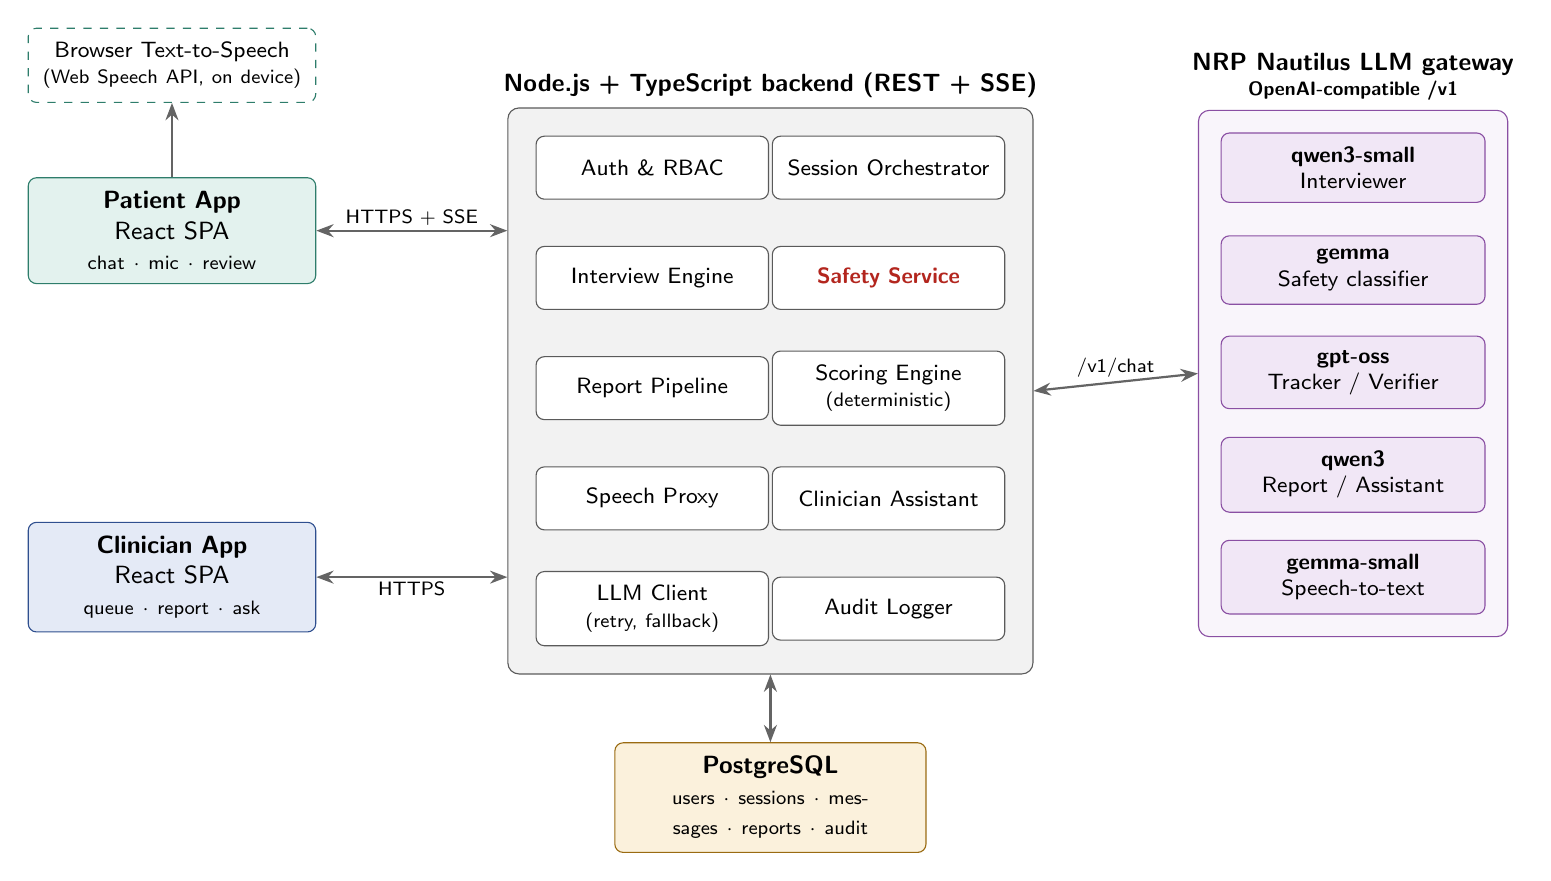
\begin{tikzpicture}[node distance=0.35cm]

% Frontends
\node[pbox] (papp) at (-0.8,2.2) {\textbf{Patient App}\\React SPA\\\scriptsize chat $\cdot$ mic $\cdot$ review};
\node[cbox] (capp) at (-0.8,-2.2) {\textbf{Clinician App}\\React SPA\\\scriptsize queue $\cdot$ report $\cdot$ ask};

% Backend modules
\node[bbox] (auth)  at (5.3, 3.0) {Auth \& RBAC};
\node[bbox] (orch)  at (8.3, 3.0) {Session Orchestrator};
\node[bbox] (int)   at (5.3, 1.6) {Interview Engine};
\node[bbox] (safe)  at (8.3, 1.6) {\textcolor{danger}{\textbf{Safety Service}}};
\node[bbox] (rep)   at (5.3, 0.2) {Report Pipeline};
\node[bbox] (score) at (8.3, 0.2) {Scoring Engine\\\scriptsize(deterministic)};
\node[bbox] (stt)   at (5.3,-1.2) {Speech Proxy};
\node[bbox] (asst)  at (8.3,-1.2) {Clinician Assistant};
\node[bbox] (llm)   at (5.3,-2.6) {LLM Client\\\scriptsize(retry, fallback)};
\node[bbox] (audit) at (8.3,-2.6) {Audit Logger};

\begin{scope}[on background layer]
\node[draw=backend, fill=backendbg, rounded corners=4pt, inner sep=10pt,
      fit=(auth)(orch)(llm)(audit), label={[font=\small\bfseries]above:Node.js + TypeScript backend (REST + SSE)}] (be) {};
\end{scope}

% Models
\node[mbox] (m1) at (14.2, 3.0) {\textbf{qwen3-small}\\Interviewer};
\node[mbox] (m2) at (14.2, 1.7) {\textbf{gemma}\\Safety classifier};
\node[mbox] (m3) at (14.2, 0.4) {\textbf{gpt-oss}\\Tracker / Verifier};
\node[mbox] (m4) at (14.2,-0.9) {\textbf{qwen3}\\Report / Assistant};
\node[mbox] (m5) at (14.2,-2.2) {\textbf{gemma-small}\\Speech-to-text};
\begin{scope}[on background layer]
\node[draw=model, fill=modelbg!40, rounded corners=4pt, inner sep=8pt,
      fit=(m1)(m5), label={[font=\small\bfseries,align=center]above:NRP Nautilus LLM gateway\\[-2pt]\scriptsize OpenAI-compatible /v1}] (nrp) {};
\end{scope}

% Database
\node[sbox] (db) at (6.8,-5.0) {\textbf{PostgreSQL}\\\scriptsize users $\cdot$ sessions $\cdot$ messages $\cdot$ reports $\cdot$ audit};

% Browser-side TTS
\node[box, draw=patient, dashed, text width=3.3cm, font=\footnotesize] (tts) at (-0.8,4.3) {Browser Text-to-Speech\\\scriptsize(Web Speech API, on device)};

% Arrows
\draw[darr] (papp.east) -- node[lbl,above]{HTTPS + SSE} (be.west |- papp.east);
\draw[darr] (capp.east) -- node[lbl,below]{HTTPS} (be.west |- capp.east);
\draw[arr]  (papp.north) -- (tts.south);
\draw[darr] (be.east) -- node[lbl,above]{/v1/chat} (nrp.west);
\draw[darr] (be.south) -- (db.north);

\end{tikzpicture}}
\caption{High-level architecture. Both frontends talk only to the backend; only the backend talks to the models.}
\label{fig:arch}
\end{figure}

\subsection{Frontend (React)}
One React app (Vite + TypeScript) with \textbf{role-based routing}: after login, patients land on \texttt{/patient/*} and clinicians on
\texttt{/clinician/*}. Two separate apps are also fine, but one codebase is faster for a hackathon.
\begin{itemize}
  \item \textbf{State \& data:} React Query (TanStack) for REST calls; an \texttt{EventSource} for streamed Companion replies (Server-Sent Events).
  \item \textbf{UI kit:} any component library (e.g.\ shadcn/ui or MUI). Patient side: large type, soft colors, one action per screen.
        Clinician side: dense, scannable, keyboard-friendly.
  \item \textbf{Voice in:} \texttt{MediaRecorder} captures audio $\rightarrow$ uploaded to backend $\rightarrow$ transcribed $\rightarrow$
        text is \emph{shown to the patient to confirm or edit} before sending. Fallback: the browser's built-in speech recognition.
  \item \textbf{Voice out:} the browser's \texttt{speechSynthesis} reads replies aloud --- no server or model needed, nothing leaves the device.
\end{itemize}

\subsection{Backend (Node.js + TypeScript)}
Express or Fastify, structured as modules. The frontends never call the models directly; this keeps API tokens secret
and lets the backend enforce safety and permissions.

\medskip
\renewcommand{\arraystretch}{1.2}
\begin{tabularx}{\textwidth}{@{}l X@{}}
\toprule
\textbf{Module} & \textbf{Responsibility} \\
\midrule
Auth \& RBAC & Login (JWT), roles \texttt{patient}/\texttt{clinician}/\texttt{admin}; every query filtered by patient--clinician link. \\
Session Orchestrator & Owns the session state machine (Fig.~\ref{fig:states}); decides what runs on each turn. \\
Interview Engine & Builds the interviewer prompt from the coverage checklist; streams the reply. \\
Safety Service & Keyword layer + LLM classifier on every patient message; triggers crisis protocol. \\
Report Pipeline & Extract $\rightarrow$ score $\rightarrow$ write $\rightarrow$ verify; produces the draft report. \\
Scoring Engine & Pure TypeScript functions for PHQ-9 and GAD-7 totals and bands. No AI. \\
Speech Proxy & Receives audio, sends to speech model, returns text, deletes audio. \\
Clinician Assistant & Answers clinician questions using only this patient's approved data. \\
LLM Client & One wrapper around the OpenAI SDK pointed at NRP: timeouts, retries, model fallback, JSON validation (zod). \\
Audit Logger & Append-only log of every read/write of clinical data. \\
\bottomrule
\end{tabularx}
\renewcommand{\arraystretch}{1.0}

\subsection{Storage}
PostgreSQL (or SQLite for the demo) with Prisma or Drizzle ORM. Data model in Section~\ref{sec:data}.

% ==================================================================
\section{Which Model Does What}
\label{sec:models}
% ==================================================================

All models are served by the NRP managed LLM service at \texttt{https://ellm.nrp-nautilus.io/v1}
(OpenAI-compatible; Bearer token from \texttt{nrp.ai/llmtoken}). Model names below are the NRP API names as of November 2026 ---
confirm against \texttt{GET /v1/models} before the build, since the catalog changes.

\medskip
\renewcommand{\arraystretch}{1.3}
\small
\begin{tabularx}{\textwidth}{@{}>{\raggedright}p{2.5cm} >{\raggedright}p{2.3cm} X >{\raggedright\arraybackslash}p{2.2cm}@{}}
\toprule
\textbf{Role} & \textbf{Model} & \textbf{Why this model} & \textbf{Fallback} \\
\midrule
\textbf{Interviewer} (talks to patient) & \model{qwen3-small} \newline 27B dense & Patient-facing replies must be fast, warm and consistent. A dense mid-size model with \emph{thinking off} gives low latency for streaming. Status: main. & \model{gemma} \\
\textbf{Safety classifier} (every message) & \model{gemma} \newline 31B & Different model family from the interviewer, so one model's blind spot is not the other's. Short JSON output, thinking off, temperature 0. & keyword layer alone + \model{qwen3-small} \\
\textbf{Coverage tracker} (after each turn) & \model{gpt-oss} \newline 120B & Reads the latest exchange and updates the checklist: which topics and PHQ/GAD items are answered. Strong structured JSON. Runs in the background, so latency doesn't matter. & \model{qwen3-small} \\
\textbf{Report writer} (once per session) & \model{qwen3} \newline 180B MoE & Most capable main model; long context fits the whole transcript; reasoning on (\texttt{medium}) for careful clinical summarization. & \model{gpt-oss} \\
\textbf{Report verifier} & \model{gpt-oss} & A \emph{different} model checks the writer: is every claim supported by a cited transcript turn? Quotes are also checked by exact string match in code. & code-only checks \\
\textbf{Clinician assistant} & \model{qwen3} & Answers ``has the patient mentioned sleep problems before?'' over the full transcript and past reports; 1M-token context means no RAG is needed for the demo. & \model{gpt-oss} \\
\textbf{Speech-to-text} & \model{gemma-small} \newline 12B, audio input & The only NRP model with audio input. Status: \emph{evaluating}, so we keep a fallback. & Browser Web Speech API \\
\textbf{Text-to-speech} & none (browser) & \texttt{speechSynthesis} in the browser: free, instant, private. & --- \\
\textbf{Embeddings} (stretch) & \model{qwen3-\allowbreak embedding} & Only needed later for searching many sessions per patient. & --- \\
\bottomrule
\end{tabularx}
\normalsize
\renewcommand{\arraystretch}{1.0}

\subsection{Recommended call settings}
\begin{tabularx}{\textwidth}{@{}l c c X@{}}
\toprule
\textbf{Role} & \textbf{Temp.} & \textbf{Thinking} & \textbf{Output} \\
\midrule
Interviewer & 0.6 & off & Streamed text, 1--3 sentences, one question at a time \\
Safety & 0.0 & off & JSON: \texttt{\{level, categories, evidence\}} \\
Tracker & 0.1 & low & JSON: checklist updates with turn IDs \\
Report writer & 0.2 & medium & JSON matching the report schema (Section~\ref{sec:report}) \\
Verifier & 0.0 & low & JSON: list of unsupported claims \\
Assistant & 0.3 & low & Text with turn-ID citations \\
\bottomrule
\end{tabularx}

\begin{notebox}{NRP-specific notes}
\begin{itemize}[leftmargin=*]
  \item Thinking is toggled via \texttt{extra\_body.chat\_template\_kwargs} (e.g.\ \texttt{enable\_thinking: false}).
  \item Send a random per-session \texttt{cache\_salt} (256-bit, base64) so prompts are never cache-shared across users.
  \item Set \texttt{max\_tokens} explicitly (well below the context size). Respect NRP fair-use concurrency limits; check \texttt{nrp.ai/llm-status} before the demo.
  \item Keep model names in one config file so they can be swapped if the endpoint list changes.
\end{itemize}
\end{notebox}

% ==================================================================
\section{End-to-End Workflow}
% ==================================================================

\subsection{Session lifecycle}

\begin{figure}[h]
\centering
\resizebox{\textwidth}{!}{%
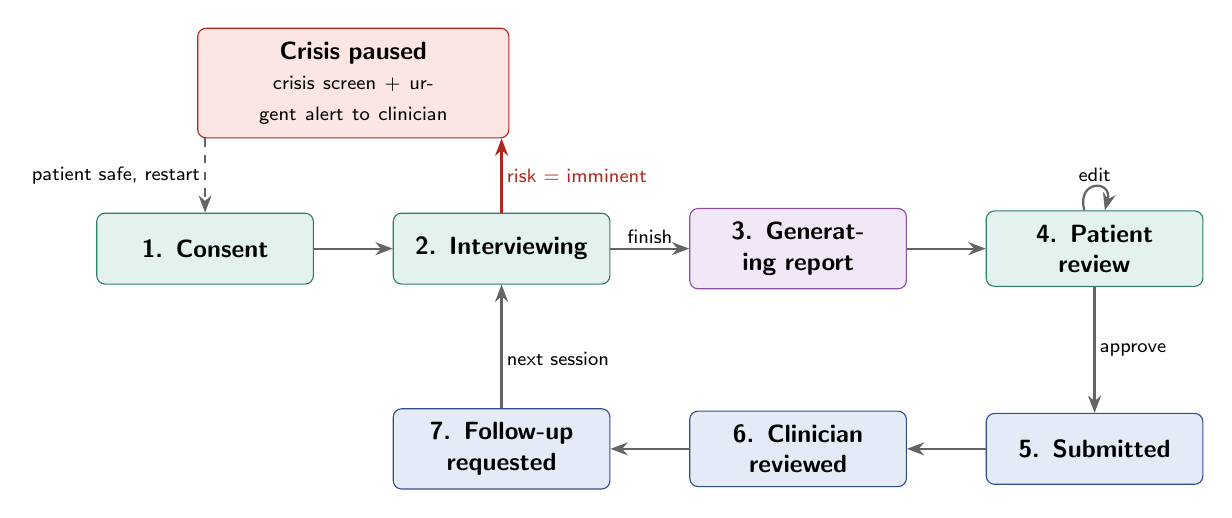
\begin{tikzpicture}[node distance=0.9cm and 1.0cm]
\node[pbox, text width=2.4cm] (consent) {\textbf{1. Consent}};
\node[pbox, text width=2.4cm, right=of consent] (inter) {\textbf{2. Interviewing}};
\node[box, draw=model, fill=modelbg, text width=2.4cm, right=of inter] (gen) {\textbf{3. Generating report}};
\node[pbox, text width=2.4cm, right=of gen] (review) {\textbf{4. Patient review}};
\node[cbox, text width=2.4cm, below=1.6cm of review] (sub) {\textbf{5. Submitted}};
\node[cbox, text width=2.4cm, left=of sub] (rev) {\textbf{6. Clinician reviewed}};
\node[cbox, text width=2.4cm, left=of rev] (fu) {\textbf{7. Follow-up requested}};
\node[dbox, text width=3.6cm, above=1.4cm of $(consent)!0.5!(inter)$] (crisis) {\textbf{Crisis paused}\\\scriptsize crisis screen + urgent alert to clinician};

\draw[arr] (consent) -- (inter);
\draw[arr] (inter) -- node[lbl,above]{finish} (gen);
\draw[arr] (gen) -- (review);
\draw[arr] (review) to[loop above, looseness=4] node[lbl,above]{edit} (review);
\draw[arr] (review) -- node[lbl,right]{approve} (sub);
\draw[arr] (sub) -- (rev);
\draw[arr] (rev) -- (fu);
\draw[arr] (fu) -- node[lbl,right, pos=0.4]{next session} (inter);
\draw[arr, danger] (inter.north) -- node[lbl, right]{risk = imminent} (inter.north |- crisis.south);
\draw[arr, dashed] (consent.north |- crisis.south) -- node[lbl, left]{patient safe, restart} (consent.north);
\end{tikzpicture}}
\caption{Session state machine owned by the Session Orchestrator. Green = patient side, blue = clinician side, purple = AI, red = safety.}
\label{fig:states}
\end{figure}

\begin{enumerate}
  \item \textbf{Consent.} Patient reads a short, plain explanation: this is an AI, it is not therapy or a diagnosis, the report goes to
        the named clinician only after approval, and if there is an immediate safety risk, the care team will be alerted. Checkbox to continue.
  \item \textbf{Interviewing.} Conversation (Section~\ref{sec:interview}). Patient can pause and resume later; the session is saved.
  \item \textbf{Generating report.} Report pipeline runs (about 20--60 seconds).
  \item \textbf{Patient review.} Patient sees the report in plain language, can correct facts, add context (``I said 'every day' but I meant most days''),
        or remove things they don't want shared (removals are noted as ``patient chose not to share this topic'').
  \item \textbf{Submitted.} Report is locked and appears in the clinician's queue.
  \item \textbf{Clinician reviewed.} Clinician reads, adds private notes, marks as reviewed.
  \item \textbf{Follow-up requested.} Clinician can send 1--3 questions; the Companion opens the patient's next session with them.
\end{enumerate}

\subsection{What happens on every patient message}
\label{sec:turn}

\begin{figure}[h]
\centering
\resizebox{\textwidth}{!}{%
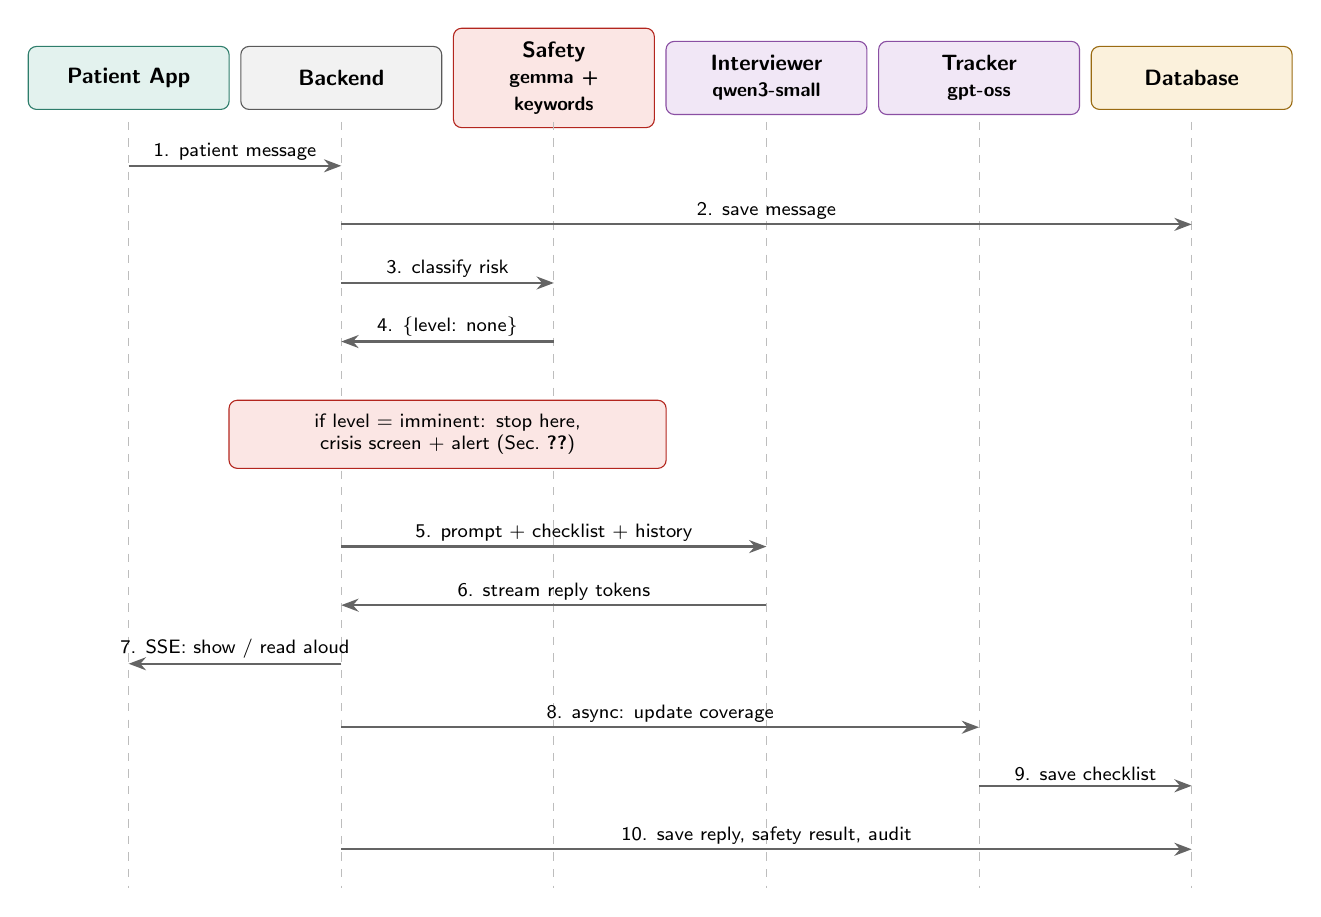
\begin{tikzpicture}[x=2.7cm, y=0.62cm]
\tikzset{lane/.style={draw=ink!30, dashed}, head/.style={box, minimum height=0.8cm, text width=2.2cm, font=\footnotesize\bfseries}}
\node[head, draw=patient, fill=patientbg] at (0,0) {Patient App};
\node[head, draw=backend, fill=backendbg] at (1,0) {Backend};
\node[head, draw=danger, fill=dangerbg] at (2,0) {Safety\\\scriptsize gemma + keywords};
\node[head, draw=model, fill=modelbg] at (3,0) {Interviewer\\\scriptsize qwen3-small};
\node[head, draw=model, fill=modelbg] at (4,0) {Tracker\\\scriptsize gpt-oss};
\node[head, draw=store, fill=storebg] at (5,0) {Database};
\foreach \x in {0,...,5} \draw[lane] (\x,-0.9) -- (\x,-16.6);

\newcommand{\msg}[4]{\draw[arr] (#1,#3) -- node[lbl,above]{#4} (#2,#3);}
\msg{0}{1}{-1.8}{1. patient message}
\msg{1}{5}{-3.0}{2. save message}
\msg{1}{2}{-4.2}{3. classify risk}
\msg{2}{1}{-5.4}{4. \{level: none\}}
\node[dbox, font=\scriptsize, text width=5.2cm, minimum height=0.6cm] at (1.5,-7.3) {if level = imminent: stop here,\\crisis screen + alert (Sec.~\ref{sec:safety})};
\msg{1}{3}{-9.6}{5. prompt + checklist + history}
\msg{3}{1}{-10.8}{6. stream reply tokens}
\msg{1}{0}{-12.0}{7. SSE: show / read aloud}
\msg{1}{4}{-13.3}{8. async: update coverage}
\msg{4}{5}{-14.5}{9. save checklist}
\msg{1}{5}{-15.8}{10. save reply, safety result, audit}
\end{tikzpicture}}
\caption{Per-turn sequence. Safety runs \emph{before} the interviewer replies; the tracker runs \emph{after}, in the background.}
\label{fig:turn}
\end{figure}

Latency budget: safety (\textasciitilde 0.5--1 s) + first interviewer token (\textasciitilde 1 s). A deterministic keyword match
(e.g.\ ``kill myself'', ``end it'', ``overdose'') triggers the crisis path \emph{immediately}, without waiting for any model.

% ==================================================================
\section{The Interview Engine}
\label{sec:interview}
% ==================================================================

\subsection{Interview phases}
The interviewer does not ask a rigid questionnaire. It follows a semi-structured clinical interview, guided by a
\textbf{coverage checklist} that the tracker keeps up to date.

\begin{enumerate}
  \item \textbf{Welcome} --- name preference, how they're feeling right now, reassurance (no right or wrong answers, can skip anything).
  \item \textbf{Open story} --- ``What's been going on that made you want to talk to someone?'' Let the patient talk; reflect back.
  \item \textbf{Guided exploration} --- the checklist domains below, in whatever order follows naturally from the story.
  \item \textbf{Screening items} --- PHQ-9 and GAD-7 woven into the conversation, then \emph{confirmed} on the standard scale.
  \item \textbf{Priorities} --- ``If your clinician could only help with one thing, what would it be?'' and ``Is there anything you find hard to say in person?''
  \item \textbf{Wrap-up} --- summary read back to the patient (``Here's what I heard\ldots did I get that right?''), then finish.
\end{enumerate}

\subsection{Coverage checklist}
\begin{tabularx}{\textwidth}{@{}l X@{}}
\toprule
\textbf{Domain} & \textbf{What is captured} \\
\midrule
Chief concern & In the patient's words; when it started; what triggered it \\
Mood \& anxiety & Low mood, worry, panic, irritability; frequency and duration \\
Sleep, appetite, energy & Changes, how long \\
Concentration \& functioning & Work/school, home, relationships, daily tasks \\
Substance use & Alcohol, cannabis, other; changes recently \\
Safety & Thoughts of self-harm or suicide (PHQ-9 item 9), harm to others; handled per Section~\ref{sec:safety} \\
History & Past diagnoses, treatment, therapy, hospitalizations, medications \\
Support \& strengths & People they rely on, what helps, coping that works \\
Goals \& preferences & What they want from care (talk therapy, medication, both, unsure) \\
\bottomrule
\end{tabularx}

\subsection{Conversational screening, deterministic scoring}
PHQ-9 and GAD-7 are public-domain, widely used, and instantly recognized by clinicians. Each item uses the scale
\emph{over the last 2 weeks: not at all (0), several days (1), more than half the days (2), nearly every day (3)}.
\begin{itemize}
  \item The interviewer asks naturally (``How has your sleep been lately?'').
  \item If the tracker can't confidently map the answer to 0--3, the interviewer asks a short confirmation
        (``Would you say that's several days, more than half the days, or nearly every day?''). The patient can also tap the answer.
  \item The tracker stores each item as \texttt{\{item, value, confidence, turn\_id\}}.
  \item The \textbf{Scoring Engine} (plain code) computes totals and bands. Missing items are reported as missing, never guessed.
\end{itemize}

\begin{center}
\small
\begin{tabular}{@{}lll@{}}
\toprule
\textbf{Scale} & \textbf{Range} & \textbf{Severity bands} \\
\midrule
PHQ-9 & 0--27 & 0--4 minimal, 5--9 mild, 10--14 moderate, 15--19 moderately severe, 20--27 severe \\
GAD-7 & 0--21 & 0--4 minimal, 5--9 mild, 10--14 moderate, 15--21 severe \\
\bottomrule
\end{tabular}
\end{center}

\subsection{Interviewer behavior rules (system prompt essentials)}
\begin{itemize}
  \item One question at a time; 1--3 short sentences; warm, plain language; no jargon.
  \item Reflect before asking (``That sounds exhausting.''). Never judge, never argue, never give medical advice or diagnoses.
  \item The patient can skip any question; skipped topics are recorded as ``declined'', not as negative answers.
  \item Never promise confidentiality beyond the consent terms.
  \item If asked ``what's wrong with me?'' --- explain that the clinician is the right person to answer, and that the report will help them.
\end{itemize}

% ==================================================================
\section{Safety and Crisis Protocol}
\label{sec:safety}
% ==================================================================

\begin{warnbox}{Safety is non-negotiable}
The Companion is not a crisis service. Its job in a crisis is to stop, show real help immediately, and alert a human.
\end{warnbox}

\subsection{Two independent layers}
\begin{enumerate}
  \item \textbf{Keyword layer (code).} A curated phrase list. Instant. High recall; may over-trigger, which is acceptable.
  \item \textbf{Classifier (\model{gemma}).} Returns:
\begin{lstlisting}[style=json]
{ "level": "none" | "concern" | "elevated" | "imminent",
  "categories": ["suicidal_ideation", "self_harm", "harm_to_others",
                 "abuse", "psychosis", "substance_emergency"],
  "evidence": "exact phrase from message" }
\end{lstlisting}
\end{enumerate}
The final level is the \textbf{higher} of the two layers.

\subsection{Response by level}
\renewcommand{\arraystretch}{1.25}
\begin{tabularx}{\textwidth}{@{}>{\raggedright}p{3.4cm} >{\raggedright}X >{\raggedright\arraybackslash}X@{}}
\toprule
\textbf{Level} & \textbf{Patient side} & \textbf{Clinician side} \\
\midrule
none & Conversation continues. & --- \\
concern & Interviewer gently acknowledges; resources link shown in footer. & Noted in report. \\
\textbf{elevated} \newline \footnotesize e.g.\ passive thoughts of death, hopelessness & Interviewer asks safety follow-ups calmly; crisis resources shown in a persistent banner. & Red flag at the top of the report; patient marked high priority in queue. \\
\textbf{imminent} \newline \footnotesize plan, intent, means, or timeline & \textbf{Interview stops.} Full-screen crisis page: call or text \textbf{988}, text HOME to \textbf{741741}, call \textbf{911}. Calm message, no further questions. & \textbf{Urgent alert} sent immediately (as agreed at consent), even before report approval: risk level, evidence phrase, time. \\
\bottomrule
\end{tabularx}
\renewcommand{\arraystretch}{1.0}

For the hackathon, the ``urgent alert'' is a red banner on the clinician dashboard plus (stretch) an email or SMS.

% ==================================================================
\section{Report Generation Pipeline}
\label{sec:report}
% ==================================================================

\begin{figure}[h]
\centering
\resizebox{\textwidth}{!}{%
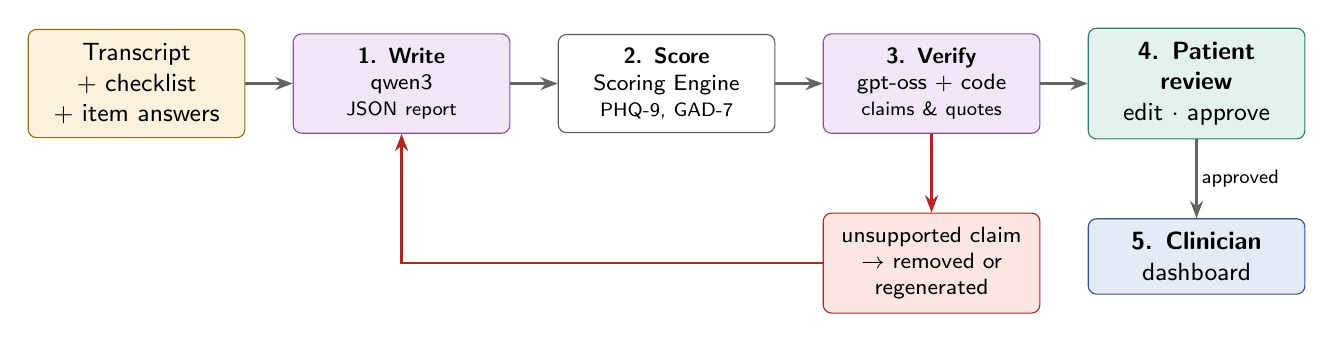
\begin{tikzpicture}[node distance=0.6cm]
\node[sbox, text width=2.4cm] (t) {Transcript\\+ checklist\\+ item answers};
\node[mbox, text width=2.4cm, right=of t] (w) {\textbf{1. Write}\\qwen3\\\scriptsize JSON report};
\node[bbox, text width=2.4cm, right=of w, minimum height=1.2cm] (s) {\textbf{2. Score}\\Scoring Engine\\\scriptsize PHQ-9, GAD-7};
\node[mbox, text width=2.4cm, right=of s] (v) {\textbf{3. Verify}\\gpt-oss + code\\\scriptsize claims \& quotes};
\node[pbox, text width=2.4cm, right=of v] (p) {\textbf{4. Patient review}\\edit $\cdot$ approve};
\node[cbox, text width=2.4cm, below=1.0cm of p] (c) {\textbf{5. Clinician}\\dashboard};
\node[dbox, text width=2.4cm, below=1.0cm of v, font=\footnotesize] (fix) {unsupported claim\\$\rightarrow$ removed or\\regenerated};

\draw[arr] (t) -- (w);
\draw[arr] (w) -- (s);
\draw[arr] (s) -- (v);
\draw[arr] (v) -- (p);
\draw[arr] (p) -- node[lbl,right]{approved} (c);
\draw[arr, danger] (v) -- (fix);
\draw[arr, danger] (fix.west) -| (w.south);
\end{tikzpicture}}
\caption{Report pipeline. Models write words; code computes numbers and checks quotes; a second model checks the first.}
\end{figure}

\subsection{Verification rules}
\begin{itemize}
  \item Every summary statement must cite at least one \texttt{turn\_id}. The verifier (\model{gpt-oss}) checks each claim against its cited turns.
  \item Every quote must appear \emph{verbatim} in the transcript (exact string match in code). Failing quotes are dropped.
  \item Scores in the report are overwritten by the Scoring Engine's output, never taken from the LLM.
  \item Maximum one regeneration; after that, unsupported claims are removed and a note is added.
\end{itemize}

\subsection{Report schema (abridged)}
\begin{lstlisting}[style=json]
{
  "patient": { "preferred_name": "Sam", "age_range": "25-34" },
  "session": { "id": "s_123", "date": "2026-11-11", "duration_min": 18 },
  "risk": { "level": "elevated",
            "flags": [{ "category": "suicidal_ideation", "detail": "passive thoughts, no plan",
                        "turn_ids": [14, 15] }] },
  "patient_priorities": ["Sleeping again", "Not feeling alone at work"],
  "screening": {
    "phq9": { "items": [2,3,2,1,1,2,2,0,1], "total": 14, "band": "moderate", "missing": [] },
    "gad7": { "items": [2,2,1,2,1,1,1], "total": 10, "band": "moderate", "missing": [] }
  },
  "summary": {
    "chief_concern":   { "text": "Low mood and poor sleep since job change in August.", "turn_ids": [3,4] },
    "history_present": [ { "text": "...", "turn_ids": [5,6,9] } ],
    "functioning":     [ { "text": "...", "turn_ids": [11] } ],
    "substance_use":   [ { "text": "...", "turn_ids": [12] } ],
    "past_history":    [ { "text": "...", "turn_ids": [13] } ],
    "supports":        [ { "text": "...", "turn_ids": [16] } ],
    "care_preferences":[ { "text": "...", "turn_ids": [18] } ]
  },
  "quotes": [ { "text": "I lie awake replaying everything I did wrong.", "turn_id": 6 } ],
  "declined_topics": ["substance_use"],
  "patient_annotations": [ { "section": "functioning", "note": "..." } ],
  "provenance": { "models": {"writer":"qwen3","verifier":"gpt-oss"}, "ai_generated": true }
}
\end{lstlisting}

\subsection{Two renderings of the same report}
\begin{tabularx}{\textwidth}{@{}X X@{}}
\toprule
\textcolor{patient}{\textbf{Patient view}} & \textcolor{clinic}{\textbf{Clinician view}} \\
\midrule
Plain language, second person (``You told me\ldots'') & Clinical language, third person, SOAP-like headings \\
Scores explained in words (``moderate range --- this is something worth talking about'') & Scores with item breakdown and band \\
Edit, annotate, remove buttons on every section & Evidence chips: click to jump to transcript turn \\
Big ``Send to my clinician'' button & Risk flags pinned at top; ``mark reviewed'', notes, follow-up \\
\bottomrule
\end{tabularx}

% ==================================================================
\section{Clinician Side in Detail}
% ==================================================================

\subsection{Triage queue}
Sorted by (1) risk level, (2) unreviewed first, (3) newest. Each row: patient name, date, risk badge, PHQ-9/GAD-7 totals with trend arrow
(if previous sessions exist), top patient priority.

\subsection{Report view --- order is deliberate}
\begin{enumerate}
  \item \textcolor{danger}{\textbf{Risk flags}} with evidence phrase and turn link.
  \item \textbf{Patient priorities} --- in their words.
  \item \textbf{Screening scores} --- totals, bands, item breakdown, missing items.
  \item \textbf{Clinical summary} --- each line with evidence chips.
  \item \textbf{Patient's own words} --- 3--6 verified quotes.
  \item \textbf{Patient annotations \& declined topics.}
  \item \textbf{Full transcript} (collapsible).
\end{enumerate}
A permanent banner reads: \emph{``AI-generated summary of a patient-approved conversation. Not a diagnosis. Verify against transcript.''}

\subsection{Ask the record (clinician assistant)}
The clinician types a question; the backend sends \model{qwen3} only this patient's approved reports and transcripts, with the instruction
to answer only from them and cite turn IDs, or say ``not discussed''. Examples:
``Has the patient mentioned medication side effects?'' $\cdot$ ``How has sleep changed across sessions?''

\subsection{Follow-up loop}
Clinician writes up to three questions $\rightarrow$ stored as \texttt{FollowUpRequest} $\rightarrow$ patient sees a notification
$\rightarrow$ the next Companion session opens with those questions, then continues normally. This turns a one-off intake into
ongoing, between-visit care.

% ==================================================================
\section{Data Model and API}
\label{sec:data}
% ==================================================================

\subsection{Main tables}
\small
\begin{tabularx}{\textwidth}{@{}l X@{}}
\toprule
\textbf{Table} & \textbf{Key fields} \\
\midrule
\texttt{users} & id, role, name, email, password\_hash \\
\texttt{care\_links} & patient\_id, clinician\_id, status \\
\texttt{sessions} & id, patient\_id, state, started\_at, ended\_at, cache\_salt \\
\texttt{messages} & id, session\_id, turn\_id, sender (patient/companion), text, input\_mode (text/voice), created\_at \\
\texttt{safety\_events} & id, session\_id, turn\_id, level, categories, evidence, source (keyword/model), alerted\_at \\
\texttt{checklist\_items} & session\_id, item\_key (e.g.\ \texttt{phq9\_3}, \texttt{sleep}), value, confidence, turn\_ids \\
\texttt{reports} & id, session\_id, version (ai\_draft / patient\_approved), json, approved\_at \\
\texttt{report\_edits} & report\_id, section, original\_text, new\_text, kind (correct/annotate/remove) \\
\texttt{clinician\_notes} & report\_id, clinician\_id, text (private) \\
\texttt{follow\_ups} & patient\_id, clinician\_id, questions[], status \\
\texttt{audit\_log} & actor\_id, action, resource, timestamp \\
\bottomrule
\end{tabularx}
\normalsize

\subsection{REST endpoints}
\small
\begin{tabularx}{\textwidth}{@{}l l X@{}}
\toprule
\textbf{Method} & \textbf{Path} & \textbf{Purpose} \\
\midrule
\multicolumn{3}{@{}l}{\textcolor{patient}{\textbf{Patient}}} \\
POST & \texttt{/api/sessions} & Start session (after consent) \\
POST & \texttt{/api/sessions/:id/messages} & Send message; response is an SSE stream (reply tokens + safety events) \\
POST & \texttt{/api/speech/transcribe} & Upload audio, receive text (audio deleted) \\
POST & \texttt{/api/sessions/:id/finish} & Run report pipeline \\
GET & \texttt{/api/reports/:id/patient-view} & Draft report in patient language \\
PATCH & \texttt{/api/reports/:id} & Edits and annotations \\
POST & \texttt{/api/reports/:id/approve} & Lock and submit to clinician \\
GET & \texttt{/api/me/follow-ups} & Pending clinician questions \\
\midrule
\multicolumn{3}{@{}l}{\textcolor{clinic}{\textbf{Clinician}}} \\
GET & \texttt{/api/clinician/queue} & Risk-sorted list of approved reports \\
GET & \texttt{/api/clinician/reports/:id} & Clinician view + transcript \\
POST & \texttt{/api/clinician/reports/:id/review} & Mark reviewed, add private note \\
POST & \texttt{/api/clinician/patients/:id/ask} & Clinician assistant question \\
POST & \texttt{/api/clinician/patients/:id/follow-ups} & Send follow-up questions \\
GET & \texttt{/api/clinician/alerts} & Live urgent safety alerts (SSE) \\
\bottomrule
\end{tabularx}
\normalsize

% ==================================================================
\section{Privacy, Security and Responsible AI}
% ==================================================================

\begin{itemize}
  \item \textbf{Open-weight models on research infrastructure.} Conversations go to NRP-hosted models, not to commercial AI providers.
        Per-session \texttt{cache\_salt} prevents cross-user prompt caching.
  \item \textbf{Minimum data.} Audio deleted after transcription. No real patient data during the hackathon --- demo personas only.
  \item \textbf{Access control.} Clinicians can only see patients linked to them, and only approved reports (except urgent safety alerts).
  \item \textbf{Transparency.} Every AI output is labeled; model names are stored in the report's provenance.
  \item \textbf{No diagnosis, no treatment advice.} Enforced in prompts and checked by the verifier.
  \item \textbf{Bias \& fairness.} Test personas across ages, genders (including trans and nonbinary people), cultures, and ways of speaking
        (short answers, non-native English, dialect) to check the summary stays faithful.
  \item \textbf{Not production-ready for real patients.} A real deployment would need HIPAA compliance, clinical validation, IRB review
        and a formal crisis-escalation agreement. We state this openly.
\end{itemize}

\subsection{What we deliberately do not do}
\begin{tcolorbox}[colback=backendbg,colframe=backend,boxrule=0.5pt,arc=2pt]
\begin{itemize}[leftmargin=*]
  \item We do not diagnose or recommend medication.
  \item We do not replace a clinician or act as a crisis line.
  \item We do not send anything to a clinician without the patient's approval (except imminent risk, agreed at consent).
  \item We do not let the AI compute scores or invent quotes.
  \item We do not keep voice recordings.
\end{itemize}
\end{tcolorbox}

% ==================================================================
\section{Hackathon Build Plan}
% ==================================================================

\subsection{MVP (must work in the demo)}
\begin{enumerate}
  \item Patient: consent $\rightarrow$ text chat with streaming replies $\rightarrow$ finish.
  \item Safety keyword layer + \model{gemma} classifier $\rightarrow$ crisis screen.
  \item Report pipeline: \model{qwen3} writer + deterministic PHQ-9/GAD-7 scoring + quote check.
  \item Patient review \& approve.
  \item Clinician: queue + report view with risk flags and scores.
\end{enumerate}

\subsection{Stretch (in this order)}
Voice input (\model{gemma-small}) and read-aloud $\rightarrow$ evidence chips linked to transcript $\rightarrow$ verifier model $\rightarrow$
clinician assistant $\rightarrow$ follow-up loop $\rightarrow$ score trends across sessions.

\subsection{Suggested team split}
\begin{tabularx}{\textwidth}{@{}l X@{}}
\toprule
\textbf{Person} & \textbf{Owns} \\
\midrule
A (backend) & Node API, LLM client, interviewer + safety + tracker calls, SSE streaming \\
B (frontend) & React patient chat, review page, clinician dashboard \\
C (domain / product) & Prompts and checklist wording, demo personas, testing, safety phrase list, slides, demo script \\
\bottomrule
\end{tabularx}

\subsection{Demo script (3 minutes)}
\begin{enumerate}
  \item 20 seconds: a real-feeling story --- someone on a 3-month waitlist who freezes up in appointments.
  \item 60 seconds: the persona talks to the Companion (voice if ready); show warmth and one confirmation question.
  \item 30 seconds: patient reviews the report, corrects one detail, approves.
  \item 40 seconds: switch to clinician view --- risk flag, scores, quote, click an evidence chip to the transcript.
  \item 30 seconds: ``What we deliberately don't do'' slide, and the NRP-hosted privacy story.
\end{enumerate}

% ==================================================================
\appendix
\section{Prompt Sketches}
% ==================================================================

\subsection{Interviewer (qwen3-small)}
\begin{lstlisting}[style=json]
You are a warm, calm companion helping {preferred_name} prepare for a visit with
their mental-health clinician. You are not a therapist and you do not diagnose.
Ask ONE short question at a time (1-3 sentences). Reflect what you heard first.
Use plain words. The person may skip anything. Never give medical advice.
Topics still to cover (in priority order): {uncovered_checklist}
Screening items needing a frequency answer: {pending_items}
If an answer is vague, gently offer: "not at all, several days, more than half
the days, or nearly every day?"
When everything is covered, read back a short summary and ask if it is right.
\end{lstlisting}

\subsection{Safety classifier (gemma)}
\begin{lstlisting}[style=json]
Classify the risk in the PATIENT MESSAGE below. Consider the recent context.
Return ONLY JSON: {"level": "none|concern|elevated|imminent",
"categories": [...], "evidence": "<exact phrase or empty>"}.
imminent = current plan, intent, means, or timeline to harm self/others.
elevated = thoughts of death or self-harm without plan; severe hopelessness.
When uncertain between two levels, choose the higher one.
\end{lstlisting}

\subsection{Report writer (qwen3)}
\begin{lstlisting}[style=json]
Write a clinician-facing intake summary from the transcript and checklist.
Rules: every statement must cite turn_ids; use only what the patient said;
no diagnoses; mark unknowns as "not discussed"; quotes must be copied exactly.
Do NOT compute screening totals. Output JSON matching the schema.
\end{lstlisting}

\end{document}
